\documentclass[submission,copyright,creativecommons]{eptcs}
\providecommand{\event}{TTC 2014} % Name of the event you are submitting to
\usepackage{breakurl}             % Not needed if you use pdflatex only.
\usepackage[utf8x]{inputenc}
\usepackage[T1]{fontenc}
\usepackage{url}
\usepackage{float}
\usepackage{textcomp}
\usepackage{wrapfig}
\usepackage{tabularx}
\usepackage{graphicx}
\usepackage{caption}
\captionsetup{compatibility=false}
\usepackage{subcaption}
\graphicspath{ {./fig/} }

\newcommand{\todo}[1]{\textbf{TODO: {#1}}}
\newcommand{\textunit}[1]{\textbf{#1.} }

% standard VIATRA stuff
\usepackage{color}
\definecolor{listinggray}{rgb}{0.92,0.92,0.92}
\definecolor{keywordcolor}{rgb}{0.5,0,0.1}
\definecolor{commentcolor}{rgb}{0,0.3,0.1}
\definecolor{stringcolor}{rgb}{0,0,1}
\usepackage{listings}
\lstdefinelanguage{viatra}
{morekeywords={@QueryBasedFeature,@Constraint,count,pattern,
    neg,find,import,true,false,or,check,job,action,state,severity,location,message,
    oclIsKindOf,self,exists,includes,invariant,class},
 sensitive=true, morecomment=[l]{//}, morecomment=[s]{/*}{*/},
 morestring=[b]{"},
}

\DeclareCaptionFormat{listing}{\colorbox[cmyk]{0, 0, 0,0}{\parbox{1.03\textwidth}{\center#1#2#3}}}
\captionsetup[lstlisting]{format=listing, singlelinecheck=false, margin=0pt}

\newcommand{\listingIQPL}[2]
{
%\renewcommand\lstlistingname{Pattern}
\lstset{backgroundcolor=\color{listinggray}}
\lstset{basicstyle=\scriptsize\ttfamily}
\lstset{commentstyle=\color{commentcolor}\ttfamily}
\lstset{stringstyle=\color{stringcolor}\ttfamily}
\lstset{frameround=tttt}
\lstset{captionpos=b}
\lstset{keywordstyle=\color{keywordcolor}\bfseries\ttfamily}
\lstset{showstringspaces=false}
\lstset{tabsize=2}
\lstset{numbers=left,numberstyle=\scriptsize\ttfamily,stepnumber=1,numbersep=5pt}
\lstset{language=viatra}
\lstset{escapeinside={(*@}{@*)}}
\lstset{breaklines=true}
\lstinputlisting[caption=#2]{#1}
}

\lstdefinelanguage{Xtend}{
 morekeywords={def,val,var,cached,case,default,extension,false,import,JAVA,WORKFLOWSLOT,let,new,null,private,create,switch,this,true,reexport,around,if,then,else,context,DEFAULT_NO_UPDATE_AND_DISAPPEAR,DEFAULT,APPEARED,DISAPPEARED,UPDATED,processor},
 keywordstyle=[2]{\textbf},
 morecomment=[l]{//}, 
 morecomment=[s]{/*}{*/}, 
 morestring=[b]",
 tabsize=2
}
\newcommand{\listingXtend}[1]{
%\lstset{backgroundcolor=\color{listinggray}}
\lstset{numbers=left,numberstyle=\tiny\ttfamily,stepnumber=1,numbersep=5pt}
\lstset{commentstyle=\color{commentcolor}\ttfamily}
\lstset{stringstyle=\color{stringcolor}\ttfamily}
\lstset{keywordstyle=\color{keywordcolor}\bfseries\ttfamily}
\lstset{breaklines=true}
\lstset{language=Xtend}
\lstset{mathescape=true}
\lstset{basicstyle=\scriptsize\ttfamily}
\lstset{escapeinside={(*@}{@*)}}
\lstset{literate=*{[guilleft]}{\guillemotleft{}}{1}{[guilright]}{\guillemotright{}}{1},}

%\lstset{literate={\-}{}{0\discretionary{-}{}{}}}
\lstinputlisting{#1}
}

\newcommand{\viatra}{\textsc{Viatra2}}
\newcommand{\incquery}{\textsc{EMF-IncQuery}}
\newcommand{\iqpl}{\incquery{} Pattern Language}

\newcommand{\defref}[1]{#1~(see~\ref{def:#1}, page~\pageref{def:#1})}
\newcommand{\figref}[1]{Figure~\ref{#1}}
\newcommand{\tblref}[1]{Table~\ref{#1}}
%\newcommand{\charef}[1]{Chapter~\ref{#1}}
\newcommand{\secref}[1]{Section~\ref{#1}}
\newcommand{\subsecref}[1]{Section~\ref{#1}}
\newcommand{\appref}[1]{Appendix~\ref{#1}}
\newcommand{\figlabel}[1]{\textsf{#1}}
\newcommand{\fl}[1]{\figlabel{#1}}

\newcommand{\code}[1]{\lstinline[basicstyle=\small\ttfamily]!#1!}
%\newcommand{\code}[1]{\lstinline[basicstyle=\small\itshape]!#1!}
\newcommand{\df}[1]{\emph{#1}}
\newcommand{\highlight}[1]{\textit{#1}}
%Defining the contract and element dependency relations
\newcommand{\edepend}[2]{\ensuremath{#1 \succ #2}}
\newcommand{\cdepend}[2]{\ensuremath{#1 \gg #2}}
\newcommand{\assign}[2]{\ensuremath{#1 \mapsto #2}}
\newcommand{\tuple}[1]{\ensuremath{\langle#1\rangle}}
\newcommand{\HEADER}{\item[\textsf{PROCEDURE}]}
% \renewcommand{\algorithmicforall}{\textbf{for each}}

\definecolor{lvl2}{rgb}{0,0.5,0}
\definecolor{lvl1}{rgb}{0,0,0.5}
\definecolor{lvl0}{rgb}{0.5,0,0}				


\makeatletter
\providecommand*{\toclevel@author}{0}
\providecommand*{\toclevel@title}{0}
\makeatother


\def\figureautorefname{Fig.}%
\def\subfigureautorefname{Fig.}%
\def\tableautorefname{Table}%
\def\partautorefname{Part}%
\def\appendixautorefname{Appendix}%
\def\chapterautorefname{Chapter}%
\def\sectionautorefname{Sec.}%
\def\subsectionautorefname{Sec.}
\def\listingautorefname{Lst.}
\def\lstnumberautorefname{Line}

\setcounter{tocdepth}{4}

\title{Movie Database Case: An \incquery{} Solution\thanks{This work was partially supported by the MONDO (EU ICT-611125) and T\'AMOP (4.2.2.B-10/1--2010-0009) projects. This research was realized in the frames of T�MOP 4.2.4. A/1-11-1-2012-0001  ,,National Excellence Program – Elaborating and operating an inland student and researcher personal support system''. The project was subsidized by the European Union and co-financed by the European Social Fund.}}
\author{
G\'{a}bor Sz\'{a}rnyas \quad 
Oszk\'{a}r Semer\'{a}th \quad 
Benedek Izs\'{o} \quad
Csaba Debreceni \and
\'{A}bel Heged\"{u}s \quad
Zolt\'{a}n Ujhelyi \quad 
G\'{a}bor Bergmann
\institute{Budapest University of Technology and Economics,\\
Department of Measurement and Information Systems,\\
H-1117 Magyar tud\'{o}sok krt. 2., Budapest, Hungary}
\email{\{szarnyas, semerath, izso, debrecenics, abel.hegedus, ujhelyiz, bergmann\}@mit.bme.hu}
}
\def\titlerunning{Movie Database Case: An \incquery{} solution}
\def\authorrunning{G. Sz\'{a}rnyas et al.}
\begin{document}
\maketitle

\begin{abstract}
This paper presents a solution for the Movie Database Case of the Transformation Tool Contest 2014, using \incquery{} and Xtend for implementing the model transformation.
\end{abstract}

\section{Introduction}

The use of automated model transformations is a key factor in modern model-driven system engineering. Model transformations allow to query, derive and manipulate large industrial models, including models based on existing systems, e.g.\ source code models created with reverse engineering techniques. Since such transformations are frequently integrated to modeling environments, they need to feature both high performance and a concise programming interface to support software engineers.

The objective of the \incquery{}~\cite{eiq-hompage} framework is to provide a declarative way to define queries over EMF models without needing to manually define imperative model traversals. \incquery{} extended the pattern language of VIATRA with new features (including transitive closure, role navigation, match count) and tailored it to EMF models~\cite{iqpl}. The semantics of the pattern language is similar to VTCL~\cite{Varro2007214}, but the adaptation of the rule language is an ongoing work.

\incquery{} is developed with a focus on \emph{incremental query evaluation} and uses the same incremental algorithm as VIATRA. The latest developments extend this concept by providing a preliminary rule execution engine to perform transformations. As the engine is under heavy development, the design of a dedicated rule language (instead of using the API of the engine) is currently subject to future work. 

Conceptually, the current execution environment provides a method for specifying graph transformations (GT) as rules, where the LHS (left hand side) is defined with declarative \incquery{} graph patterns, defined in \iqpl{}~\cite{iqpl} and the RHS (right hand side) as imperative model manipulations formulated in the Xtend programming language~\cite{xtend}. The rule execution engine is also configured from Xtend code.

One case study of the 2014 Transformation Tool Contest describes a movie database transformation~\cite{Horn14}. The main characteristics of the transformation related to the application of \incquery{} are that i) it only adds new elements to the input model (i.e.\ couples and groups are created without modifying the input model), and ii) it is non-incremental (i.e.\ adding a new group with a rule will not affect the applicability of rules).

The rest of the paper is structured as follows: \secref{sec:overview} gives an overview of the implementation, \secref{sec:solution} describes the solution including design decisions, benchmark results, and \secref{sec:conclusion} concludes our paper.


\section{Architecture Overview}
\label{sec:overview}

The overview of the rule-based solution is illustrated in \figref{fig:overview}. The input of the transformation is a \emph{movie model}. The result is a \emph{transformed movie model} containing additional model elements, including various groups (couples and $n$-cliques) and their average rating~\cite{Horn14}. The transformation runs in a Java application, that uses \emph{pattern matchers} provided by \incquery{} and model modification code specified in Xtend.
The model \emph{modifications} are performed over EMF resources, while the pattern matcher \emph{monitors} the resources to incrementally update match sets.
The application initially reads the input movie database resource, creates the output resources (organizing them into a resource set), then executes the transformation, and finally serializes the results into files.

\begin{figure}
	\centering
	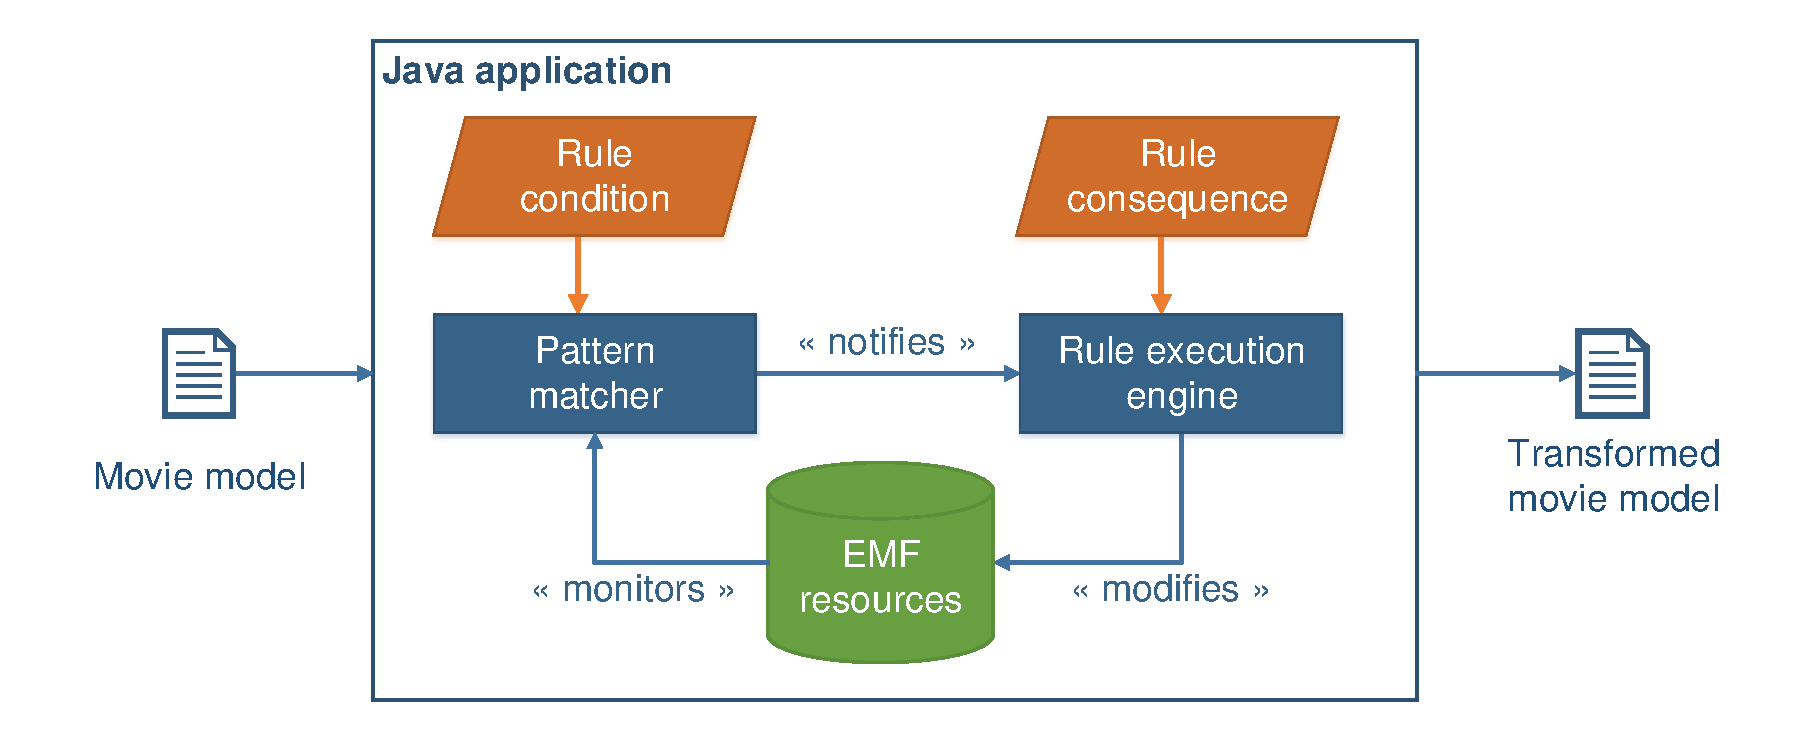
\includegraphics[width=.9\textwidth]{architecture.pdf}
	\caption{Overview of the specification and runtime.}\label{fig:overview}
\end{figure}

The whole solution is implemented in two languages. Rule conditions are formulated as \incquery{} graph patterns, while the rule consequences (model manipulations) in Xtend. Since the advanced transformation constructs of \incquery{} are tailored for event-driven (incremental) execution, the current solution only uses pattern matchers to access query results, without additional constructs.

%\begin{wrapfigure}{r}{0.6\textwidth}
%  \vspace{-150pt}
%  \begin{center}
%	\includegraphics[width=.6\textwidth]{metamodel_v2.pdf}
%  \end{center}
%  \caption{Our extended metamodel.}\label{fig:metamodel}
%\end{wrapfigure}

\section{Solution}
\label{sec:solution}

\subsection{Specification}

In the provided Ecore model, no containment hierarchy is used and all objects are held in the \textsf{contents} list of the EMF resource. However, this also means that the performance of the transformation can be affected by the resource implementation used (since it will determine the implementation of the list operations).

For performance considerations, we used an extended version of the metamodel, which has a \textsf{Root} object. %(see \figref{fig:metamodel}). 
This object serves as a container for all \textsf{Group}, \textsf{Movie} and \textsf{Person} objects. According to our experiments, this increases the speed of the pattern matching by a factor of two.

We ensured that our solution works with the models provided and also persists outputs in a format that does not include the root element. This way, the transformation part of our solution is independent of resource implementation (binary, UUID-based, regular XMI, etc.).

\subsection{Patterns and Transformations}

\subsubsection{Task 1: Generating Test Data}
\label{t1}

The synthetic test data is generated in Xtend (see Listing~\ref{app:xtend:task1}). The code tightly follows the specification defined in the case description~\cite{Horn14}.
Since the task is simple model construction without any querying, \incquery{} is not used in this task. 

\begin{figure}[!t]
    \begin{minipage}{.32\textwidth}
	\listingXtend{./src/generator_p1.xtend}
	\end{minipage}    
    \begin{minipage}{.32\textwidth}
	\listingXtend{./src/generator_p2.xtend}
	\end{minipage}    
    \begin{minipage}{.32\textwidth}
	\listingXtend{./src/generator_p3.xtend}
	\end{minipage}    
\end{figure}

\subsubsection{Task 2: Finding Couples}
\label{t2}

Couples are listed with the following pattern:

\begin{figure}[!t]
    \begin{minipage}{.50\textwidth}
	\listingIQPL{./src/couple.eiq}{Couple}
	\listingIQPL{./src/commonMoviesOfCouple.eiq}{CommonMoviesOfCouple}
    \end{minipage}
    \hspace{0.03\textwidth}
    \begin{minipage}{.48\textwidth}
	\listingIQPL{./src/groupSize.eiq}{GroupSize}
	\listingIQPL{./src/clique-3.eiq}{Clique-3}
    \end{minipage}
\end{figure}

Note that the \textsf{cast} pattern returns the names of persons that play in a given movie. This is important since the names of the persons can be used to avoid symmetric matches in the \textsf{personsToCouple} pattern by sorting.
The \textsf{Couple} objects are created and configured in Xtend (see \textsf{createCouples} in line~\ref{xform:createCouples} of Listing~\ref{app:xtend:xform}). This includes setting the \textsf{p1} and \textsf{p2} references using a \textsf{personName} pattern and computing the \textsf{commonMovies} by simple set intersection operators (\textsf{retainAll}).

\subsubsection{Task 3: Computing Average Rankings}
\label{t3}

The average rankings are computed in Xtend by calculating the mean of the \textsf{rating} attributes of a couple's common movies (see \textsf{calculateAvgRatings} in line~\ref{xform:calculateAvgRatings} of Listing~\ref{app:xtend:xform}). The movies are enumerated with the following pattern:


\subsubsection{Extension Task 1: Compute Top-15 Couples}
\label{et1}

This task is mostly implemented in Xtend (see \textsf{topGroupByRating} in line~\ref{xform:topGroupByRating} and \textsf{topGroupByCommonMovies} in line~\ref{xform:topGroupByCommonMovies} of Listing~\ref{app:xtend:xform}), however, it uses the \textsf{groupSize} pattern in order to filter the groups with the particular number of members.


This pattern uses the \textsf{count find} construct which computes the number of matches for a given pattern. 
Additionally, specific comparators are used to sort and determine the top-15 lists by rating or number of common movies (see Listing~\ref{app:xtend:comparator}). 

\begin{wrapfigure}{r}{0.4\textwidth}
  \vspace{-48pt}
  \begin{center}
	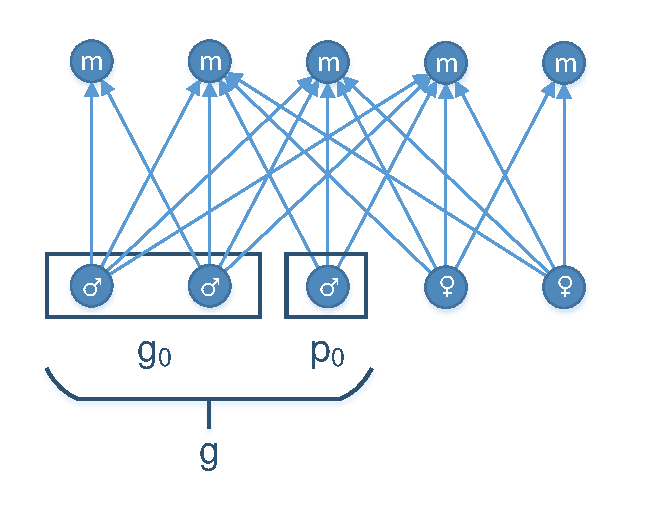
\includegraphics[width=.4\textwidth]{positive-pattern.pdf}
  \end{center}
  \caption{Matching 3-clique groups in the positive test pattern. $g_0$ is a couple.}\label{fig:positive-pattern}
  %\vspace{-52pt}
\end{wrapfigure}

\subsubsection{Extension Task 2: Finding Cliques}
\label{et2}

The pattern for finding cliques is implemented similarly to the \textsf{personsToCouple} pattern~\ref{t2}. The pattern for 3-cliques is defined as follows:


The creation of cliques is done similarly to couples (see \textsf{createCliques} in line~\ref{xform:createCliques} of Listing~\ref{app:xtend:xform}). However, this pattern has a redundant check constraint, as $P_1 < P_2$ and $P_2 < P_3$ already imply $P_1 < P_3$. This works as a hint for the query engine and allows it to filter the permutation of the results (e.g.\ $(a_2, a_1, a_3), (a_1, a_3, a_2), \ldots)$) earlier.

To achieve high query performance, patterns for 4- and 5-cliques are defined manually. For larger cliques ($n > 5$), patterns could be automatically generated using code generation techniques.


\paragraph{General solution for $n$-cliques.} We also provide the outline for a more general solution (for arbitrary $n$ values). For the sake of clarity, we will refer to couples as 2-cliques. In this approach, the cliques are built iteratively. Suppose we already have all $k$-cliques in the graph (e.g.\ we already added the 2-, 3-, 4- and 5-cliques with the previous patterns). To get the $(k+1)$-cliques, we look for a group $g_0$ and a person $p_0$ that (i) have at least 3 movies in common, (ii) $ g = g_0 \cup \left\{p_0\right\} $ is a group that is not a subset of any other groups (see Figure~\ref{fig:positive-pattern}).


Formally, (ii) can be expressed as $ \left(\not\exists g'\right): g \subseteq g' $. Using $ g = g_0 \cup \left\{p_0\right\} $, we derive the following expression $\left(\not\exists g'\right): \left(g_0 \subseteq g'\right) \wedge \left(p \in g'\right)$. The $g_0 \subseteq g'$ expression can be formulated as follows: $\left(\forall p_0 \in g_0\right): p_0 \in g'$. As the \iqpl{} does not have a universal quantifier, we rewrite this using the existential quantifier: $\left(\not\exists p_0 \in g_0\right): p_0 \not\in g'$.


The resulting expression for condition (ii) is the following: $\left(\not\exists g'\right): \left(\left(\not\exists p_0 \in g_0\right): p_0 \not\in g'\right) \wedge \left(p \in g'\right)$. This is equivalent to the following \incquery{} pattern:

\begin{figure}[!t]
    \begin{minipage}{.50\textwidth}
      \listingIQPL{./src/subset.eiq}{Subset}
      \listingIQPL{./src/clique_p1.eiq}{Clique}
	\end{minipage}
    \hspace{0.03\textwidth}
    \begin{minipage}{.48\textwidth}
      \listingIQPL{./src/clique_p2.eiq}{Clique}
	\end{minipage}
\end{figure}

Based on the \textsf{subsetOfGroup} pattern, we may implement the \textsf{nextClique} pattern like follows:


Given a model containing all $k$-cliques, the \textsf{nextClique} pattern is capable of determining the $(k+1)$-cliques. While this solution is functionally correct, it only works for very small input models and hence is omitted from our implementation.

\subsubsection{Extension Task 3: Compute Average Rankings for Cliques}
\label{et3}

The average rankings are computed the same way as in \emph{task 3} (section~\ref{t3}).

\subsubsection{Extension Task 4: Compute Top-15 Cliques}
\label{et4}

The top 15 average rankings are computed the same way as in \emph{extension task 2} (section~\ref{et2}).

\subsection{Optimizations}

To increase the performance of the transformations, we used some optimizations.

\begin{itemize}
  \item After the matcher engine produced the initial result set, the engine is turned off. This way, we spare the cost of incrementally maintaining the result set. As the transformation is non-incremental, this does not affect the result of the performance. 
  \item The common movies of the two \textsf{Person} objects are computed from Xtend instead of \incquery{}.
  \item The patterns for 3-, 4- and 5-cliques are implemented manually.
\end{itemize}
 
We looked for \emph{common subpatterns} and extracted them into separate patterns. This results in better performance as the engine can reuse the pattern for each occurrence, and makes the query definition file easier to maintain. For an example, see the \textsf{cast} pattern in~\ref{app:pattern}.

\subsection{Build Automation}

Our solution was developed in the Eclipse IDE. While it is fully functional in Eclipse, it can also be compiled with the Apache Maven~\cite{Maven} build automation tool. This offers a number of benefits, including easy portability and the possibility of continuous integration. The build process uses the Tycho Maven plug-in~\cite{tycho} to build the Eclipse plug-ins defined in the project.

\subsection{Benchmark Results}

The implementation was benchmarked in the SHARE cloud, on an Ubuntu 12.04 64-bit operating system running in a VirtualBox environment. The virtual machine used one core of an Intel Xeon E5-2650 CPU and had 6 GB of RAM.

The benchmark used Maven to build the binary files. The transformations were ran in a timeout window of 10 minutes.

\subsection{Synthetic model}

Results are displayed in \figref{fig:benchmark-results}. The diagram shows the transformation times for creating couples and cliques for synthetic models. The results show that the transformations run in near linear time.

The dominating factor of the running time is the initialization of the query engine. However, after initialization, creating groups can be carried out efficiently.

Furthermore, our experiments showed that the limiting factor for our solution is the memory consumption of the incremental query engine. Given more memory, the solution is capable of transforming larger models as well.

\begin{figure}
	\centering
	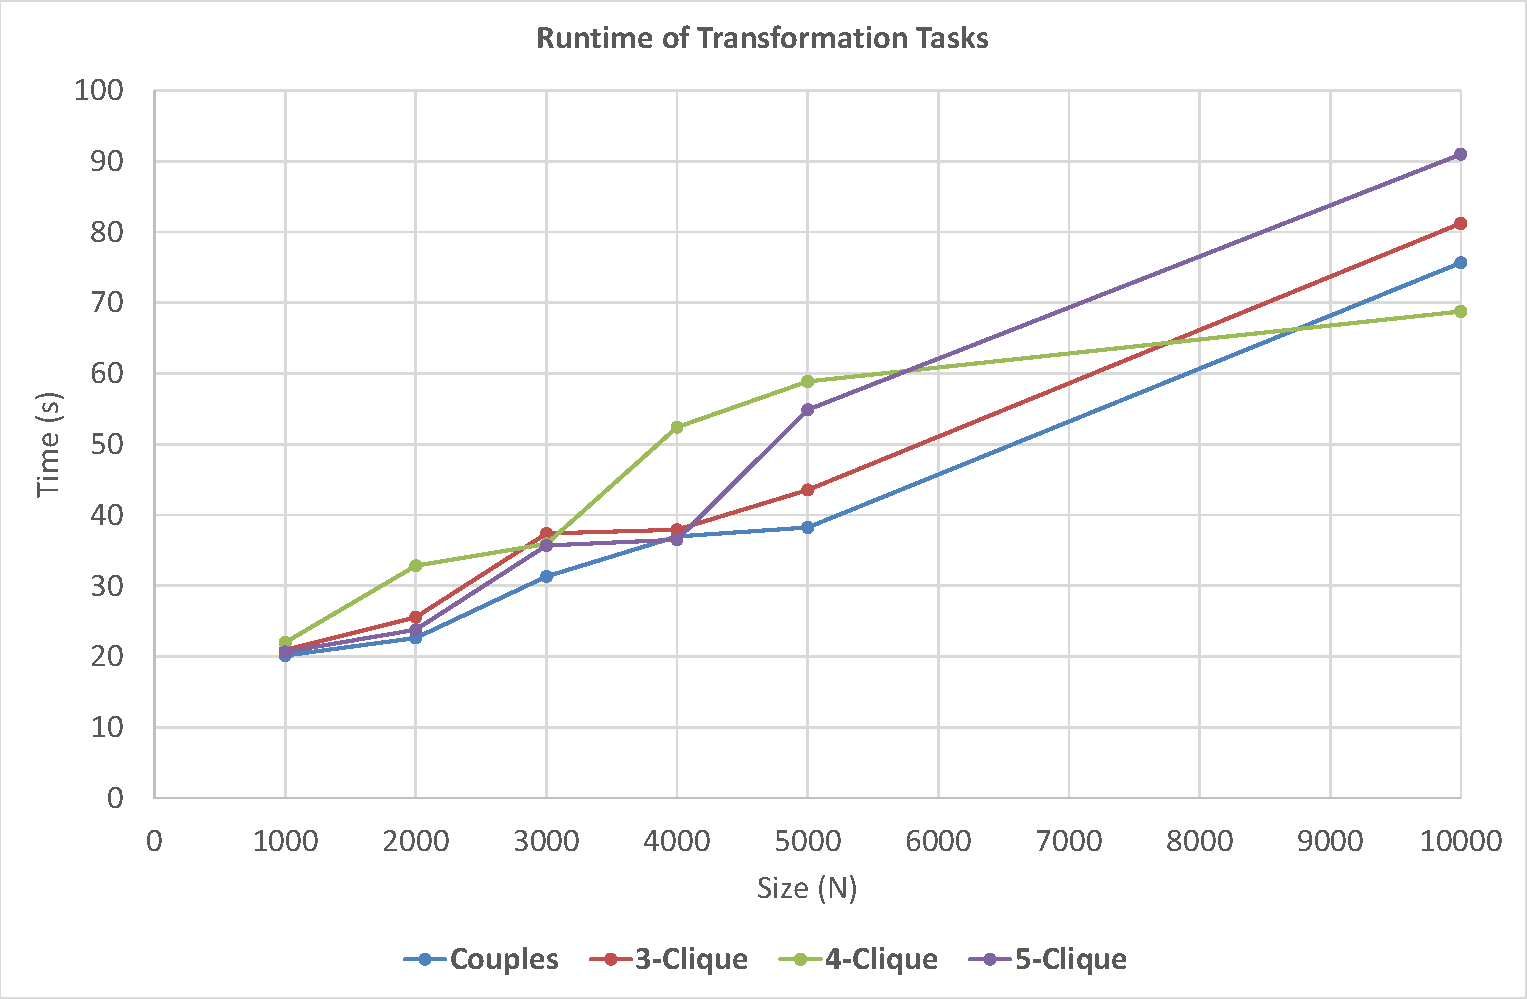
\includegraphics[width=.9\textwidth]{results-full.pdf}
	\caption{Benchmark results.}\label{fig:benchmark-results}
\end{figure}

\subsection{IMDb model}

In the given time range and memory constraints, the transformation of the IMDb model could only generate the couples and 3-cliques for the smallest instance model. Finding the couples took 3 minutes, while finding 3-cliques took 6. However, in case of a live and evolving model, our solution is capable of incrementally running the transformation which in practice results in near instantaneous response time.

\subsection{Transformation Correctness and Reproducibility}

The transformation runs correctly for the provided test cases on SHARE\footnote{\url{http://is.ieis.tue.nl/staff/pvgorp/share/?page=ConfigureNewSession&vdi=Ubuntu12LTS_TTC14_64bit_TTC14-EIQ-imdb.vdi}}, and the source code is also available in a Git repository\footnote{Homepage: \url{https://git.inf.mit.bme.hu/w?p=projects/viatra/ttc14-eiq.git} (use the \texttt{anonymous} user with no password), clone URI: \texttt{https://anonymous@git.inf.mit.bme.hu/r/projects/viatra/ttc14-eiq.git}}. The results of the transformations were spot-checked for both synthetic and IMDb models.  

\subsection{Tool Support for Debugging and Refactoring}

As the transformation is written in two languages, debugging and refactoring is dependent on the tooling for these languages and the capabilities of the query engine. 

Xtend and the \incquery{} pattern editors are based on Xtext, and while provide some refactoring operations. Declarative \incquery{} graph patterns cannot be efficiently debugged at runtime. However, smaller instance models can be loaded into the \emph{Query Explorer} view, which is very handy to the debug matches of the patterns. The engine controller code can be debugged and refactored as well, as it is implemented in Java. Debug messages of the execution engine can be turned on, which prints useful messages about rule firings and activations. Firings of the transformation operations can be debugged by placing breakpoints in the Xtend code.



\section{Conclusion}
\label{sec:conclusion}

In this paper we have presented our implementation of the Movie Database Case. The solution is based on \incquery{} which is used as a model query engine. Because its dedicated rule language is yet to be implemented, the transformation rules are defined in Xtend.

The transformation is specified using declarative graph pattern queries over EMF models for rule preconditions, and Xtend code which can be executed to obtain the desired effect of the rule.


%\newpage 

\bibliographystyle{eptcs}
\bibliography{bib/ttc14}

%\clearpage
%\appendix
%\section{Appendix -- Movie Database Case Transformation Code}
\label{app:xform}

\subsection{\incquery{} Graph Patterns}
\label{app:pattern}

\listingIQPL{./src/imdb.eiq}

%\newpage

\subsection{Xtend Code}

\subsubsection{Generator code}
\label{app:xtend:task1}

\listingXtend{./src/generator.xtend}

\subsubsection{Transformation code}
\label{app:xtend:xform}
\listingXtend{./src/transformation.xtend}

\subsubsection{Comparator code for top-15}
\label{app:xtend:comparator}
\listingXtend{./src/comparator.xtend}



\end{document}
